\section{Examplary Two Player Game Sequence}
\subsection{Starting the Game}
The main menu is created and added to the world by requet of the FBGame instance,
returning the reference to the FBGame. This menu offers a few options to start 
a game session. Clicking on the "Start 2 Player Game" button results in the message
\lstinline!FBGame>>startGames:! to be send with the parameter two.
%
\begin{figure}[bt]
  \begin{center}
    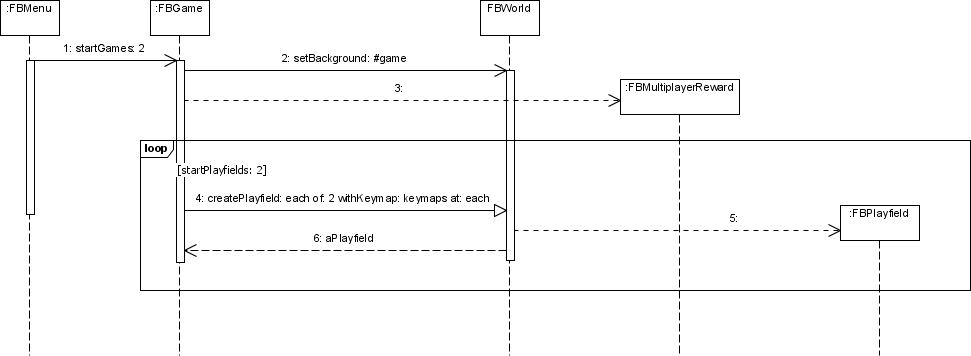
\includegraphics[width=\linewidth]{images/Starting2PlayerGame.png}
  \end{center}
  \caption{Starting a 2 Player Game}
  \label{fig:Starting2PlayerGame}
\end{figure}
%
The FBWorld instance catches any keyboard interrupt and hands it over to the game. If
this keystroke is not registered in the games keymap (e.g. it's not bound to pause or
exit) it is handed over to all the playfields, which may ignore it or act accordingly -
if it's in their keymap. As we assume in this example, that the key that was pressed is
bound to the shoot command of the playfield, it picks the shoot event from the keymap.
Therefor the playfield will ask it's cannon to shoot. The cannon sends the message shoot:
to the playfield it belongs to, with it's current angle as parameter. The playfield
sends the message fly: to it's current ball so it takes of with the given angle.
The ball keeps flying until ti collides, as described in section \ref{sec:collisionmap}.
As soon as the ball got stuck, it notifies the playfield controller, which in turn notifies
the playfield.
%
\begin{figure}[bt]
  \begin{center}
    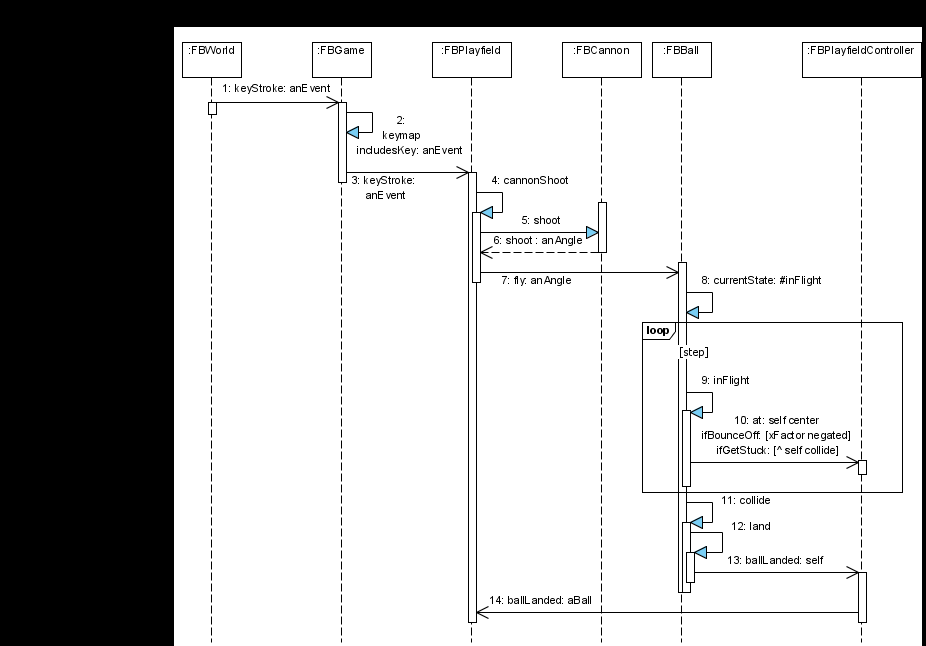
\includegraphics[width=\linewidth]{images/ShootingABall.png}
  \end{center}
  \caption{Shooting a Ball}
  \label{fig:ShootingABall}
\end{figure}
%
%
\begin{figure}[bt]
  \begin{center}
    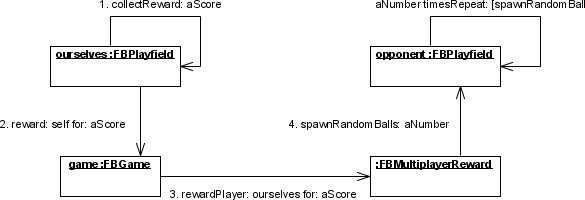
\includegraphics[width=\linewidth]{images/RewardingAPlayer.png}
  \end{center}
  \caption{Rewarding a Player for his Actions}
  \label{fig:RewardingAPlayer}
\end{figure}
%